\chapter{Présentation générale}
\label{chap:premierchapitre}

\section{Le pitch}
\textbf{Life Invader} est un jeu dans lequel vous incarnerez un nouveau réseau social. Celui-ci a pour but de prendre le contrôle sur toutes les informations privées de chaque personne sur terre afin de servir un but obscur !

\section{Description de l'application}

Vous venez de créer votre nouveau réseau social. Il est temps de le développer, d'augmenter le nombre d'utilisateurs actifs. Pour cela, tous les coups sont permis ! Négociez des contrats publicitaires, faites un pacte avec une nation pour obtenir des fonds contre un accès aux données de vos membres. Créez une association pour fournir internet dans des pays du tiers-monde afin que leurs habitant puisse avoir accès à vos produits !

Plusieurs types de victoire sont possibles ! Arriverez-vous à promouvoir votre réseau à l'ensemble de la population mondiale active ? Deviendrez-vous la société avec le plus grand capital au monde ? Découvrez les autres types de victoire en arpentant Life Invader !

\section{Cible}

Tous les détenteurs d'un ordinateur équipé de JAVA. La cible est un joueur occasionnel qui soit désire jouer rapidement, soit désire prendre son temps pour aller plus loin. Elle représente les jeunes de 15 à 45 ans.

\section{Fonctionnalités}

\begin{itemize}
    \item L'interface Graphique (GUI) sera fortement inspiré de celui du jeu PlagueInc. (Figure \ref{plagueIncMap}, Page \pageref{plagueIncMap})
    \item Concernant l'interface console, celle-ci sera composée de différents menus afin d'obtenir des informations sur le monde et des répercussions des actions sur celui-ci.
    
    \item Il faudra gérer votre réputation pour que les utilisateurs continuent à s'inscrire et qu'ils restent actifs.
    
    \item A travers les différents menus :
    
    \begin{itemize}
        \item il est possible de gérer son réseau social à travers trois type d'actions :
    
        \begin{itemize}
            \item \textbf{Growth} : Qui permet d'augmenter le nombre d'utilisateur par le biais d'actions marketing
            \item \textbf{Security} : Qui permet d'améliorer la sécurité de votre réseau social afin de ne pas subir des attaques d'autres états ou concurrents
            \item \textbf{Black Ops} : Cette catégorie d'actions consiste à faire du \textbf{Lobbying} auprès d'états pour assouplir la régulation du marché, de signer des contrats secrets avec des agences de renseignement,...
        \end{itemize}
        \end{itemize}
        \item{Un \textbf{live feed} interactif pour augmenter le réalisme du jeu. Celui-ci évolue en fonction des actions de l'utilisateur}
        \item Pour faire évoluer le réseau, il faut dépenser de l'argent. Celui-ci est gagné de différentes manières : 
        \begin{itemize}
            \item Suivant les mise à jours de votre réseau, vous obtiendrez régulièrement des revenus de manière automatique
            \item Périodiquement, des actions marketing auront lieu partout dans le monde, cliquez dessus et vous obtiendrez un bonus d'utilisateur et d'argent
            \item Grâce au menu blackops vous obtiendrez certaines facilités (Moins de taxes, ...) et également une grosse compensation d'argent. Mais votre réputation en prendra un coup
        \item Tous les réseaux sociaux présents dans la partie rencontrerons périodiquement des attaques de la part d'états, de hackers et de concurrents.
        \item Un concurrent commencera en même temps que vous (AI ou autre joueur), il disposera exactement des mêmes fonctionnalités, avantage/défaut que les vôtres.
    \end{itemize}
    
\end{itemize}
\begin{figure}
\begin{center}
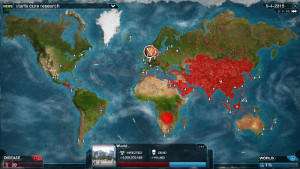
\includegraphics{images/plagueIncMap.jpg}
\end{center}
\caption{L'interface du jeu Plague Inc - \copyright NDemic Creations }
\label{plagueIncMap}
\end{figure}
%%% Local Variables: 
%%% mode: latex
%%% TeX-master: "cahierDesCharges"
%%% End: 